% !TEX root = ../main.tex

\chapter{Mathematical preliminaries} % Main chapter title
\label{Chapter2}


\section{General Relativity}

General Relativity is the theory of space, time and gravitation developed by Einstein in 1915. 
It introduced a new viewpoint on gravity and it's relation with the fabric of spacetime, a \emph{manifold} that bounded our three spatial dimensions with dimension of time, which was a concept that challenged our deeply ingrained and intuitive notions of nature partially because the mathematical background need to understand the precise formulation of theory was unfamiliar to much of the Physics community at the time.

This formulation corresponds to a field theory which the main object of study is the metric of the manifold, $g=g_{\mu\nu} \dd x^\mu \dd x^\nu$, and inherits diffeomorphism invariance, which was at the core of definition of differential manifolds. Firstly, the theory was left aside because of the numerous complicated coupled nonlinear equations, but the astronomical discovery of compact and highly energetic objects in the 1950s breaded new interest into the somewhat dormant GR, mainly because it was thought that these quasars and compact X-ray sources had suffered some form of gravitational collapse or that strong gravitational fields were present.
Soon after, the modern theory of gravitational collapse was developed and the first solutions of BHs were discovered in the mid-1960s, including the Schwarzschild and Kerr BHs.

The theory of GR can be elegantly described in the form of the Hilbert action
\begin{align}
    S_{H} = \frac{1}{16\pi} \int \dd^4 x \sqrt{-g} \,R ~,
    \label{eq2:actionGR}
\end{align}
where $g=\det(g_{\mu\nu})$ and $R$ corresponds to the Ricci scalar.
Naturally, the first solutions corresponded to pure gravity, usually designated as vacuum solutions, which obey
\begin{align}
    R_{\mu\nu} = 0 ~.
    \label{eq2:vacuumGR}
\end{align}
Despite their simplicity, they enjoy some very fascinating nontrivial properties. 
One of which is the existence of an event horizon, a surface that separates two causally disconnected regions of spacetime.

Particularly, in this work we will also include electromagnetic (massless, neutral) wave interactions, which are described by the Maxwell action
\begin{align}
    S_{EM} = - \frac{1}{4} \int \dd^4 x \sqrt{-g} \,F_{\mu\nu} F^{\mu\nu} ~,
     \label{eq2:actionEM}
\end{align}
where $F_{\mu\nu}$ is the Maxwell tensor. Variation of both actions, $\delta(S_H + S_{EM}) = 0$, result in two field equations
\begin{align}
    \nabla_\mu F^{\mu\nu} &= 0 ~, \label{eq2:maxwellEM} \\
    R_{\mu\nu} - \frac{R}{2} g_{\mu\nu} &= 8 \pi T_{\mu\nu} \label{eq2:EM+GR}  ~.
\end{align}
The first equation is just the usual of Maxwell equation in curved spacetime.
The latter is the Einstein field equation, which reflects the backreaction of the electromagnetic waves into the geometry through the presence of EM stress-energy tensor
\begin{align}
    T_{\mu\nu} = F_{\mu\lambda} F_{\nu}{}^{\lambda} - \frac{1}{4} g_{\mu\nu} F^2  ~.
    \label{eq2:stressenergyEM}
\end{align}
These equation completely describe the system, but the problem is analytically untreatable, so will be resorting to perturbation theory, considering the field $A^\mu$ to be small. 
This is a very good approximation, since near the gravitational field of stellar-mass BHs  is considerably strong compared with radiation emitted by nearby astrophysical sources.
As the stress-energy tensor is quadratic in the fields, $T_{\mu\nu}\sim\mathcal{O}(A^2)$, then we can ignore the backreaction and the field equations for the metric $g_{\mu\nu}$ reduce to~\eqref{eq2:vacuumGR}.
Therefor we need only to focus on the Maxwell equation in a static background.
In order to to able to solve this equations we will resort to the Newman-Penrose formalism, which is suited to study any kind of radiation in curved spacetime.


\section{Kerr black hole}

It was generally accepted that a perfectly spherical symmetrical star would collapse to a Schwarzschild BH. Although it was not known the effect of a slightest amount o angular momentum on a gravitational collapse of a star. Finding a metric with intrinsic rotation could give insight to such problem. Due to the lack of spherical symmetry, the problem became much harder, and took roughly 50 years after Schwarzschild's discovery to find a metric for a rotating body. Imposing symmetries to the final metric were essential to solve the field equation.


\subsection{Spacetime symmetries}

If we represent our spacetime by $(\mathcal{M}, g_{\mu\nu}, \psi)$, then the pullbash $f^*$ of the diffeomorphism $f:\mathcal{M}\rightarrow\mathcal{M}$, would give us the same physical system $(\mathcal{M}, f^* g_{\mu\nu}, f^* \psi)$.
Since diffeomorphisms are just active coordinate transformations, such concept may raise some confusion, as we don't seam to obtain no new information to work with. 
Almost all physics theories are coordinate invariant, as is Newtonian mechanics and Special Relativity, but in such theories there is a preferable coordinate system, while the same does not hold true for GR.
An analogies can be made with the path integral formalism in QFT, where special consideration is taken when summing all field configurations in order to not overcount indistinguishable configurations, as is the case of gauge field theories.
A similar ambiguity can occur in GR, where two apparently different solutions which can be related by a diffeomorphism and are actually ``the same'', so we must be careful when deriving and analyzing any geometries.

Despite the added complexity of Einstein's field equations, it is still possible to find exact nontrivial solutions in a systematic way by considering spacetimes with symmetries with the use of Killing vector fields.
A vector field $\xi$ that obeys
\begin{align}
    \mathcal{L}_\xi  g = 0  
    \label{eq2:killing}
\end{align}
is called a Killing field. Locally, this expression reduces to $\nabla_\mu \xi_\nu + \nabla_\nu \xi_\mu = 0$.

A \emph{stationary} solution implies the existence of a Killing vector $k$ that is asymptotically timelike, $k^2<0$, therefore allows us to normalize our vector such that $k^2 \rightarrow -1$. 
Unlike the case of the static spacetime, a stationary metric does not show invariance under reversal of the time coordinate, which is natural considering a system with angular momentum. 
Futhermore, a solution is also \emph{axisymmetric}, due to the presence of a asymptotically spacelike Killing field $m$ whose integral curves are closed. A solution is stationary and axisymmetric if both symmetries are present, along with commuting fields, $[k , m] = 0$, \emph{i.e.} rotations along with the axis of symmetry commute with time translations. The commutativity of the fields implies the existence of a set of coordinates, $(t,r,\theta,\phi)$, such that
\begin{align}
    k = \frac{\partial}{\partial t} ~, \qquad m = \frac{\partial}{\partial \phi} ~.
    \label{eq2:tPhiKilling}
\end{align}
As for direct implication of this choice of chart, components of the metric stay independent of $(t,\phi)$, in virtue of~\eqref{eq2:killing},
\begin{align}
    (\mathcal{L}_m g)_{\mu\nu} = \frac{\partial g_{\mu\nu}}{\partial \phi} = 0 ~,
    \label{eq2:lieMetricTPhi}
\end{align}
with the same holding true for $k$, hence we can write $g_{\mu\nu} = g_{\mu\nu}(r,\theta)$. 

One of the major applications of Killing vectors is to find conserved charges associated with the motion along a geodesic spanned by field.
These quantities are defined by taking the geodesics to regions space that are asymptotical flat, where the geometry does not affect the observer.
In the case of Kerr solution, we have two Killing vectors, $k$ and $m$, which are naturally associated with the total mass $M$ and angular momentum $J$ of the BH, respectively.
This is usually done by evaluating the Komar integrals~\cite{Heusler1996, Wald2010}, which can be written a covariant way as
\begin{alignat}{6}
    M = &&\, -\frac{1}{8 \pi} & \int_{S^2_\infty} \star \dd k^\flat \,& = &&\, \frac{1}{4} & \lim_{r\to\infty}  \int_0^\pi \dd\theta \sqrt{-g} \, g^{t\alpha} g^{r\beta} g_{t[\alpha,\beta]} ~, \label{eq2:komarMass} \\
    J = &&\, \frac{1}{16 \pi} & \int_{S^2_\infty} \star \dd m^\flat \,& = &&\, - \frac{1}{8} & \lim_{r\to\infty}  \int_0^\pi \dd\theta \sqrt{-g} \, g^{t\alpha} g^{r\beta} g_{\phi[\alpha,\beta]} ~, \label{eq2:komarSpin}
\end{alignat}
where the usual notation $k^\flat = g(k, \,\cdot\,) = g_{\mu\nu} k^\mu \dd x^\nu$ transforms a vector into a one-form and $\star : \Omega^{p}(\mathcal{M})\to\Omega^{4-p}(\mathcal{M})$ is the Hodge dual map. In order to complete the integration in the last step is assumed (\ref{eq2:tPhiKilling}) and (\ref{eq2:lieMetricTPhi}), keeping $(t,r)$ constant. According to the widely accepted of \emph{no-hair conjecture}~\cite{Carter1971}, these two quantities completely define a stationary (neutral) BH. 


\subsection{Kerr-Child coordinates}

Naturally, Kerr wasn't the only after such solution.
Many presented other metrics to approximately describe a rotating star. 
Most of the solutions were modified one-parameter modification to Schwarzschild that were not flat in case of the standard case. 
Simply using stationary and axisymmetric symmetries and then solving the Einstein's equations clearly wouldn't sufice.

Kerr success originated in of Petrov's classification of spacetimes, which used the algebraic properties of the Weyl tensor to distinguish the solutions in 3 types, along with some subcases.
Kerr assumed that his solution would have the same classification as Schwarzschild's, which associated with the gravitational fields of isolated massive objects, such as stars and BHs. 
From this assumption, using GR spinor techniques in Newman-Penrose formalism, a only then imposing the Killing vectors in~\eqref{eq2:tPhiKilling}, was possible to find a new solution. Kerr's metric appear in his original paper in the form
\begin{align}
    \begin{split}
        g = &- \left(1 - \frac{2 M r}{\rho^2} \right) (\dd v - a \sin^2\theta \dd \chi )^2 \\
        &+ 2  (\dd v - a \sin^2\theta \dd \chi )  (\dd r - a \sin^2\theta \dd \chi ) \\
        &+ \rho^2 (\dd \theta^2 + \sin^2\theta \dd \chi^2 ) ~,
    \end{split}
    \label{eq2:KerrIngoingEF}
\end{align}
where $a$ is a parameter, $M$ is the Komar mass and $\rho^2 = r^2 + a^2 \cos^2\theta$. Naturally the stationary Killing vector is $\partial_v$ and $\partial_\chi$ is the axial field, which implies that $J = a M$.

Taking the limt of $a\to0$, we reduce the metric to the Schwarzschild solution in ingoing Eddington-Finkelstein coordinates, $(v,r,\theta,\chi)$, which are useful to study ingoing (to the horizon) geodesics and remove the horizon coordinate singularity. If a given metric has singularities, then it is not trivial to identify if is a physical singularity or just an artifact resultant of choice of the chart, which can simply be removed by a better choice of coordinates. 
That being said, this raises the dificulty of finding the essential singularities.
The best way to look to these singularities is to compute curvature scalar quantities, and if they diverge in one chart then they diverge on all charts.
Since any BH is just a vacuum solution, then the Ricci scalar vanishes, $R=0$, so we resort to the Kretschmann scalar,
\begin{align}
    R_{\mu\nu\rho\sigma} R^{\mu\nu\rho\sigma} = \frac{48 M (r^2 - a^2\cos^2\theta) \left[ (r^2 - a^2\cos^2\theta) ^2 - 16 r^2 M^2 a^2\cos^2\theta \right] }{(r^2 + a^2\cos^2\theta)^6} ~,
    \label{eq2:KerrKretschmann}
\end{align}
that diverges for $\rho^2=0$.
The Schwarzschild singularity, $r=0$, is replaced with the Kerr singularity $(r,\theta)=(0,\pi/2)$. It is not clear who is the geometry of the Kerr singularity if we interpret $r$ and $\theta$ as being part of the ordinary spherical coordinates. Although the metric is singular, considering $(t,r,\theta)$ constant and then the limit of $r\to\infty$, the metric
\begin{align}
    g_{\rvert\mathrm{singularity}} \sim a^2 \dd \chi^2 ~
    \label{eq2:KerrKretschmann}
\end{align}
is reduced to the line element of $S^1$, a \emph{ring singularity} of radius $a$, only when $\theta=\pi/2$. This result implies that only approaching the a Kerr BH through the equatorial plane we may reach the singularity $\rho^2=0$. 

The Kerr-Child ``cartesian'' form, 
\begin{align}
    \begin{split}
        g = &- \dd \tilde{t}^2 + \dd x^2 + \dd y^2 + \dd z^2 \\
        &+ \frac{2 M r^3}{r^4 + a^2 z^2} \left[ \dd \tilde{t} + \frac{r (x \dd x + y \dd y) - a (x \dd y - y \dd x)}{r^2+a^2} + \frac{z}{r} \dd z \right]^2 ~,
    \end{split}
    \label{eq2:KerrChild}
\end{align}
is useful to really observe the ring singularity. In this metric, $r$ is no longer a coordinate but a function of this chart coordinates $(\tilde{t},x,y,z)$. We can relate the The Kerr-Child metric to the original Kerr solution, using
\begin{align}
    \tilde{t} = v - r ~, \qquad x+ i y = (r -i a) e^{i \chi} \sin\theta ~,\qquad z=r\cos\theta ~,
    \label{eq2:InEFtoKChild}
\end{align}
which implies that $r(x,y,z)$ is implicitly given by
\begin{align}
    r^4 - (x^2+y^2+z^2-a^2)r^2 -a^2 z^2 = 0 ~.
    \label{eq2:rConditionKChild}
\end{align}

\begin{figure}[h]
    \centering
    \begin{subfigure}[c]{0.45\textwidth}
        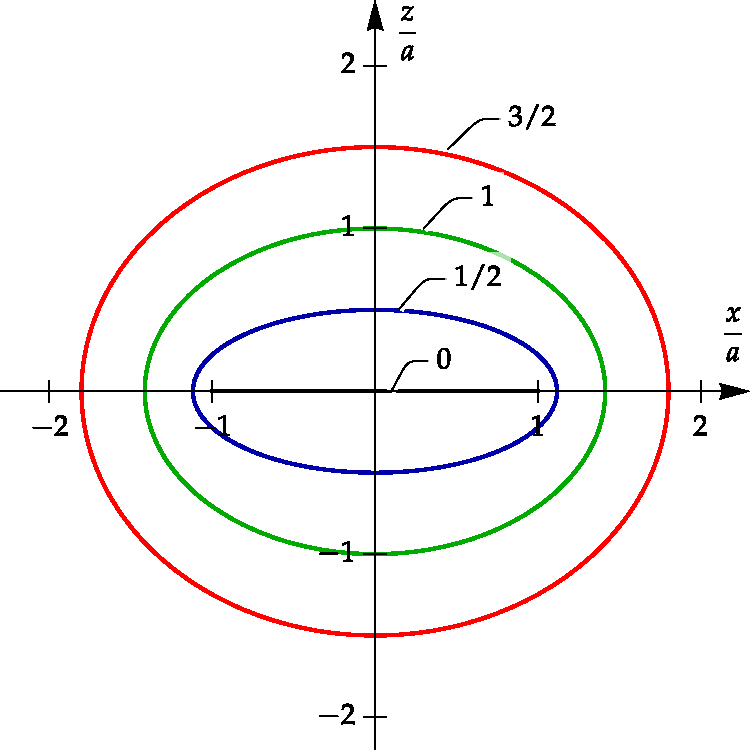
\includegraphics[width=\textwidth]{kerrchild2d}
    \end{subfigure}
    \hspace{1cm}
    \begin{subfigure}[c]{0.35\textwidth}
        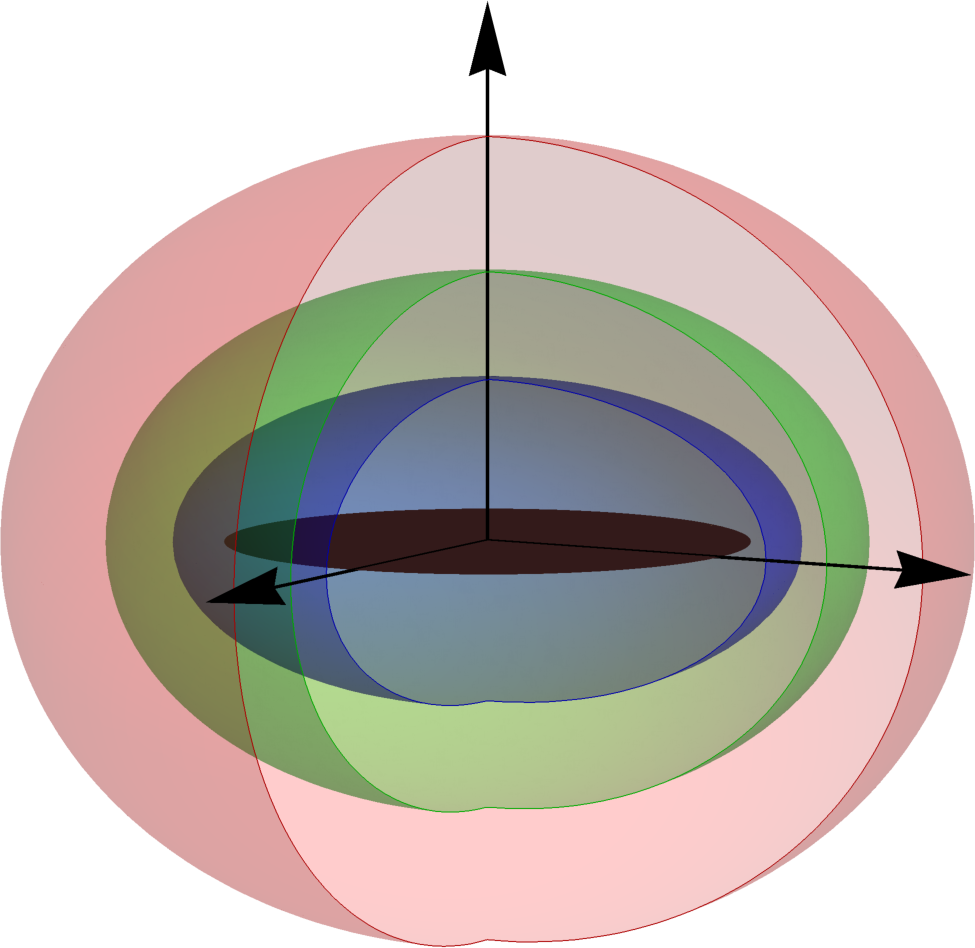
\includegraphics[width=\textwidth]{kerrchild3d}
    \end{subfigure}
    \caption{Contour plots of the surface $r(x,y,z)$ for constant values of $0,\,1/2,\,1,\,3/2$, in the Kerr-Child ``cartesian'' coordinates. The left plot is the intersection with $z=0$ plane with the 3D representation (right) that spotlights the ring singularity.}\label{fig2:kerrchild}
\end{figure}

This condition deserves a more in-depth analysis.
For increasing $r$, the surfaces obeying~\eqref{eq2:rConditionKChild} approximates perfect spheres as the geometry get more and more flat, as is observed in (\ref{eq2:KerrChild}).
Minkowsky flat space is also guaranteed for $M=0$.
On the other hand, as we approach the singularity on $z=0$ and $x^2+y^2 = a^2$ the surfaces become oblate (for the strict inequality, the singularity is removable).
Such remarks are visually demonstrated in~\fref{fig2:kerrchild}.

Even thought both metrics $r>0$, there is no mathematical reason to restrict $r$ strictly to positive values.
Particularly for Kerr-Child, hypersurfaces of constant $r$ can be represented also by $-r$. 
This means that this chart can be analytically extended to regions where $r<0$.
From this procedure and a proper collage of charts it is possible to achieve a \emph{maximally extended} solution, with gives mathematical access to new spacetime regions, even tough most of them show unphysical properties.


\subsection{Boyer-Linquist coordinates}

Considering the problem in hand, the most suitable coordinates for work with the NP formalism, are the Boyer-Linquist coordinates
\begin{align}
    \begin{split}
        g = &- \left(\dd t - \frac{2 M r}{\rho^2} \right) \dd t^2 - 2 a \sin^2\theta \frac{(r^2+a^2-\Delta)}{\rho^2} \dd t \dd \phi \\
        &+ \frac{(r^2+a^2)^2- \Delta a^2 \sin^2\theta}{\rho^2} \sin^2\theta \dd\phi^2 + \frac{\rho^2}{\Delta} \dd r^2 + \rho^2 \dd \theta^2 ~,
    \end{split}
    \label{eq2:KerrBL}
\end{align}
where we define $\Delta=r^2-2 M r + a^2$. In order to show that these corresponds to the same solution, the change of coordinates
\begin{align}
    \dd v= \dd t + \frac{r^2+a^2}{\Delta} \dd r ~, \qquad \dd\chi = \dd\phi + \frac{a}{\Delta} \dd r ~.
    \label{eq2:InEFtoBL}
\end{align}
This coordinates are usually referred as ``Schwarzschild like'', as it takes the spherical static case in standard curvature coordinates when setting $a=0$. 
Time inversion symmetry is characteristic of static Schwarzschild spacetime, but not for Kerr. 
Nevertheless, this specific form is invariant under the inversion $(t,\phi)\to(-t,-\phi)$, also known as the \emph{circular condition}, an intuitive notion from physical systems with angular momentum. 
This discrete symmetry eliminates most of the off-diagonal components of the BL metric, $g_{tr} = g_{\phi r} = g_{t \theta} = g_{\phi \theta} = 0$, making it the simplest to perform calculations.

The one-form, $n = \dd r$, defines normal vectors to $r$ constant surfaces. It is easy to show that $n^2 = g^{rr}$, which implies that $n$ is null when $\Delta=0$, defining null hypersurfaces at 
\begin{align}
    r_\pm = M \pm \sqrt{M^2 - a^2} ~,
    \label{eq2:KerrRadius}
\end{align}
singularities at $g_{rr}$ which we know to be removable.
Hence, from a stationary observer point of view, a massless particle on an ingoing null geodesic would spiral around the BH for a infinite time, as the coordinate $t\to\infty$, never reaching $r=r_{+}$.
This surface is the event horizon of the Kerr BH, which separates two causally disconnected regions of spacetime, therefore we only need to focus on the region physical region $r>r_{+}$. The surface at $r=r_{-}$ is also called a Cauchy horizon.
The expression for the event horizon also raises limitations for the amount of angular momentum a physical BH can have. We must have $|a| < M$, otherwise $\Delta$ would lack of any real roots, which would lead to a essential \emph{naked singularity}, reachable in a finite observable time, which is forbidden by the \emph{Weak Cosmic Censorship}.   

Event tough most of the Kerr BH properties were shown, there is was no result so far showed some kind of rotation.
First, consider the quantity $\xi_\mu u^\mu$, where $u^\mu$ is the four-velocity vector and $\xi^\mu$ is a Killing field.
Being aware of the geodesic equation, $u^\nu \nabla_\nu u^\mu = 0$, this quantity is conserved along geodesics, \emph{i.e.}
\begin{align}
    u^\nu \nabla_\nu ( \xi_\mu u^\mu ) = u^\mu u^\nu \nabla_\nu \xi_\mu = \frac{u^\mu u^\nu }{2} ( \nabla_\mu \xi_\nu + \nabla_\nu \xi_\mu ) = 0 ~,
    \label{eq2:geodesicKilling}
\end{align}
due to Killing~\eqref{eq2:killing}. As a result, geodesics of a free particle in Kerr geometry will be characterized by two constants
\begin{align}
    -\epsilon &= k^\mu g_{\mu\nu} \frac{\dd x^\nu}{\dd \tau} ~, \qquad \ell = m^\mu g_{\mu\nu} \frac{\dd x^\nu}{\dd \tau} ~,
    \label{eq2:geodesicConsts}
\end{align}
where $\tau$ is the affine parameter fo the geodesic. These quantities can be interpreted the energy per mass and angular momentum per mass of the particle, respectively. Due to the circular form of the BL metric, the metric components of the coordinates $(t,\phi)$ define a product decomposition, providing the separation of previous equations, specified for the equatorial plane,
\begin{align}
    \dot{t} &= \frac{1}{\Delta} \left[ (r^2+a^2 +\frac{2 M a^2}{r})\epsilon - \frac{2 M a}{r} \ell \right] ~, \\
    \dot{\phi} &= \frac{1}{\Delta} \left[ \frac{2 M a}{r} \epsilon +\left( 1- \frac{2 M}{r} \right) \ell \right]  ~.
    \label{eq2:geodesicPhiT}
\end{align}
The final equation for the geodesic is provided by the line element (\ref{eq2:KerrBL}), which becomes also a first order ODE, after substitution of $\dot{t}$ and $\dot{\phi}$.

If an test particle starts with $\ell=0$ relative to a zero angular momentum observer (ZAMO), then we can get the angular velocity $\Omega$, as measured at infinity
 \begin{align}
    \Omega = \frac{\dot{\phi}}{\dot{t}} = - \frac{g_{t\phi}}{g_{\phi\phi}} = \frac{2 a M}{r^3 + a^2 (2 M+r)} ~.
    \label{eq2:geodesicKilling}
\end{align}
Asymptotically we obtain $\Omega=0$, consistent with the ZAMO measurements. But for a finite distance, infalling geodesics are forced to co-rotate with the BH. Particularly, at the event horizon, $r=r_+$, on finds that
 \begin{align}
    \Omega_H = \frac{a}{2 M r_+} = \frac{a}{2 M (M+\sqrt{M^2-a^2})} ~.
    \label{eq2:geodesicKilling}
\end{align}


% \begin{figure}[h]
%     \centering

%     \begin{subfigure}[c]{0.45\textwidth}
%         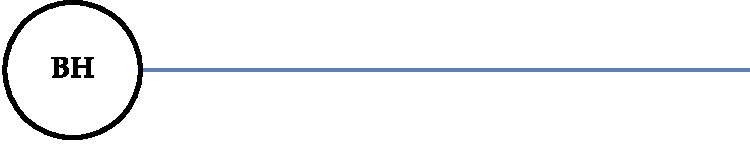
\includegraphics[width=\textwidth]{geodKerr_0_0}
%         \caption{~$a=0 ~, ~~ \ell=0$}
%     \end{subfigure}
%     \hspace{1cm}
%     \begin{subfigure}[c]{0.45\textwidth}
%         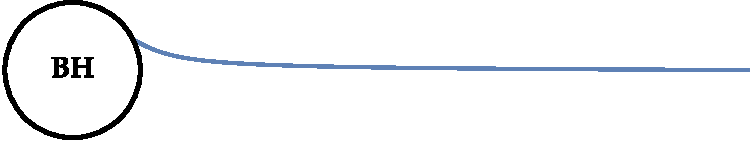
\includegraphics[width=\textwidth]{geodKerr_99_0}
%         \caption{~$a=0.99 ~, ~~ \ell=0$}
%     \end{subfigure}

%     \begin{subfigure}[c]{0.45\textwidth}
%         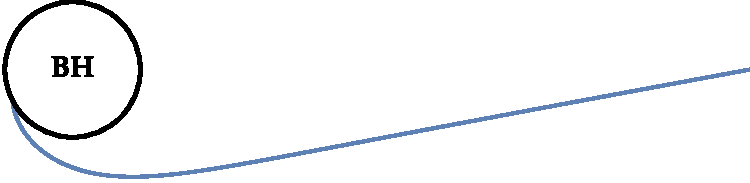
\includegraphics[width=\textwidth]{geodKerr_0_-5}
%         \caption{~$a=0 ~, ~~ \ell=-5 \epsilon$}
%     \end{subfigure}
%     \hspace{1cm}
%     \begin{subfigure}[c]{0.45\textwidth}
%         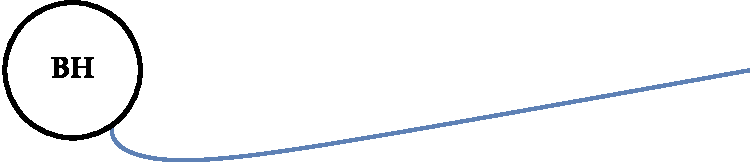
\includegraphics[width=\textwidth]{geodKerr_99_-5}
%         \caption{~$a=0.99 ~, ~~ \ell=-5 \epsilon$}
%     \end{subfigure}
    
%     \caption{Kerr Child}\label{fig2:kerrchild}
% \end{figure}

\subsection{Ergoregion and Penrose process}



From now on, all results will be provided using BL coordinates.

\section{Newman-Penrose formalism}

\subsection{Kinnersly tetrad}
\subsection{Spin coefficients}
\subsection{Maxwell equations}


\cleardoublepage